\documentclass[10pt,twocolumn,letterpaper]{article}

\usepackage{cvpr}
\usepackage{times}
\usepackage{epsfig}
\usepackage{graphicx}
\usepackage{amsmath}
\usepackage{amssymb}
\usepackage{caption}
\usepackage{subcaption}

\usepackage[breaklinks=true,bookmarks=false]{hyperref}

\cvprfinalcopy

\def\cvprPaperID{****}
\def\httilde{\mbox{\tt\raisebox{-.5ex}{\symbol{126}}}}

\begin{document}

%%%%%%%%% TITLE
\title{Identify the category of foliar diseases in apple trees}

\author{Muhammad Arham Bin Tariq\\
Ravensburg-Weingarten University of Applied Sciences\\
Weingarten, Germany\\
{\tt\small muhammadarhambin.tariq@hs-weingarten.de}
}

\maketitle
%\thispagestyle{empty}

%--------------------Abstract---------------------------------------------%
\begin{abstract}
In order to keep apple plants safe from diseases, it is important to detect the disease quickly and accurately. Manual detection could be slow and inaccurate, which results in losses and other health effects. However machine learning based algorithms can speed up the process and provide high accuracy. For this purpose a data set was made available on Kaggle with real-life images of multiple apple foliar diseases. To automate the classification of the plant diseases a convolutional neural network was then trained.
\end{abstract}

%--------------------Introduction------------------------------------------%
\section{Introduction}
Detecting diseases in apple plants manually could be a slow and inaccurate process which results in huge losses. To automate this process a data set with different images from apple plants having different diseases was provided on kaggle. The goal was to classify each plant into the category of the disease it had or to the category of being healthy. For this goal machine learning is the best approach, where a deep neural network is trained on the images captured. The model learns from these images and is then able to classify the image. 


%---------------------Dataset----------------------------------------------%
\section{Exploring the Data set}
The Data set provided on Kaggle contained 3651 manually captured, real-life symptom images of multiple apple foliar  diseases, with variable illumination,  angles,  surfaces,  and  noise. Out of 3651, 1820 images were used for training and the rest of 1821 images were to be used for testing. Each image belonged to one of the following catogeries: 
\begin{itemize}
\item Healthy (the plant does not have any disease)
\item Rust
\item Scab
\item Multiple Diseases (the plant has more than one disease)
\end{itemize}
Figure 1 shows examples of images belonging to these four classes. \cite{kaggle}
\begin{figure}
\begin{subfigure}{.22\textwidth}
  \centering
  % include first image
  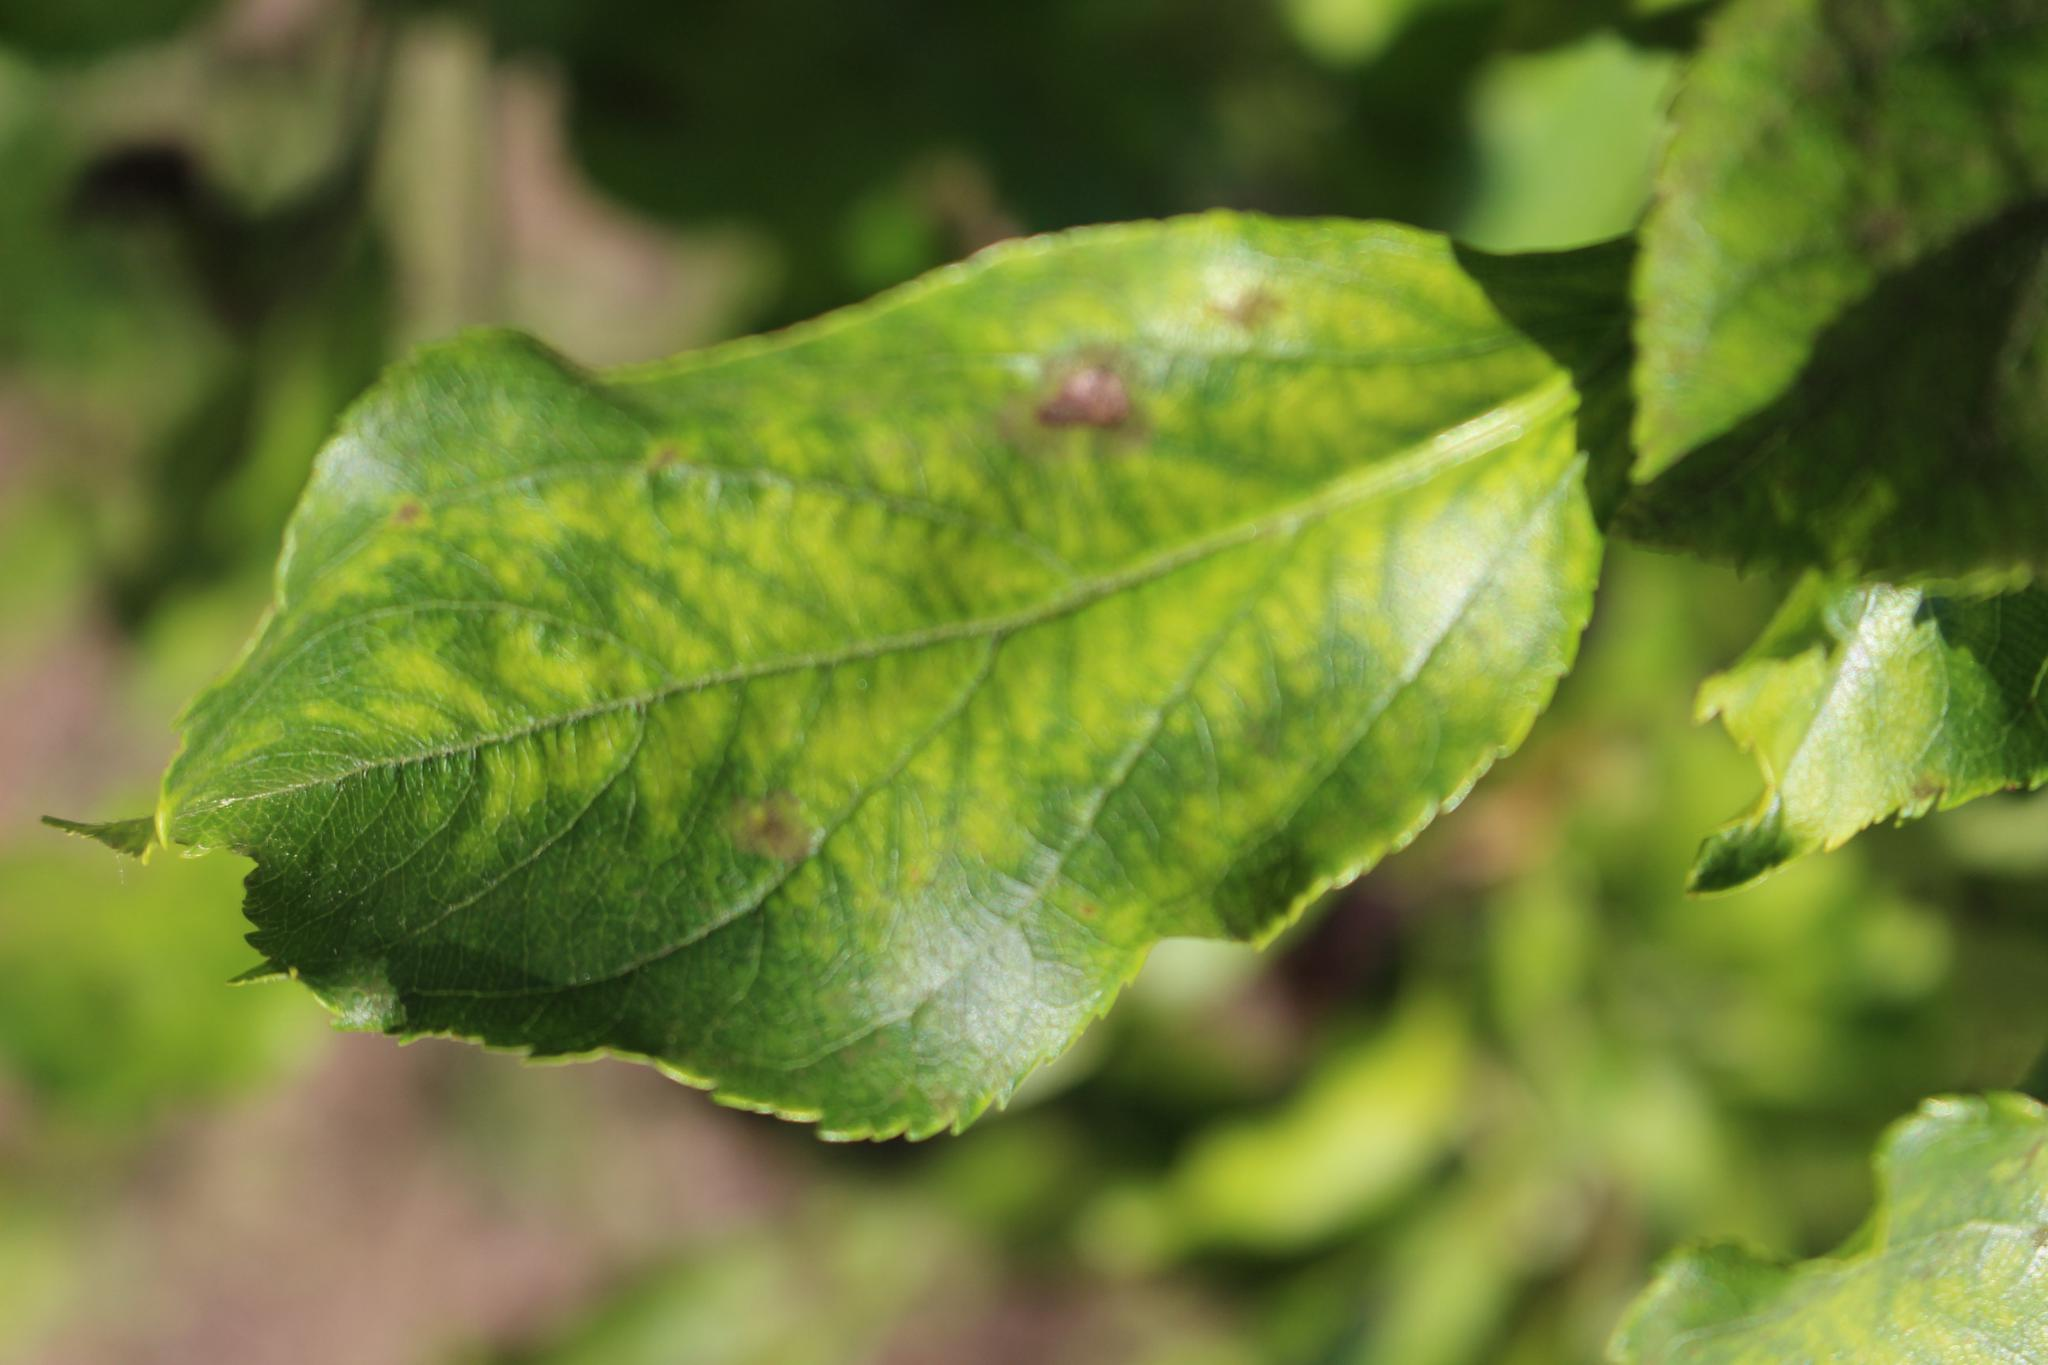
\includegraphics[scale= 0.05]{images/scab.jpg}  
  \caption{Plant with scab}
  \label{fig:sub-first}
\end{subfigure}
\begin{subfigure}{.22\textwidth}
  \centering
  % include second image
  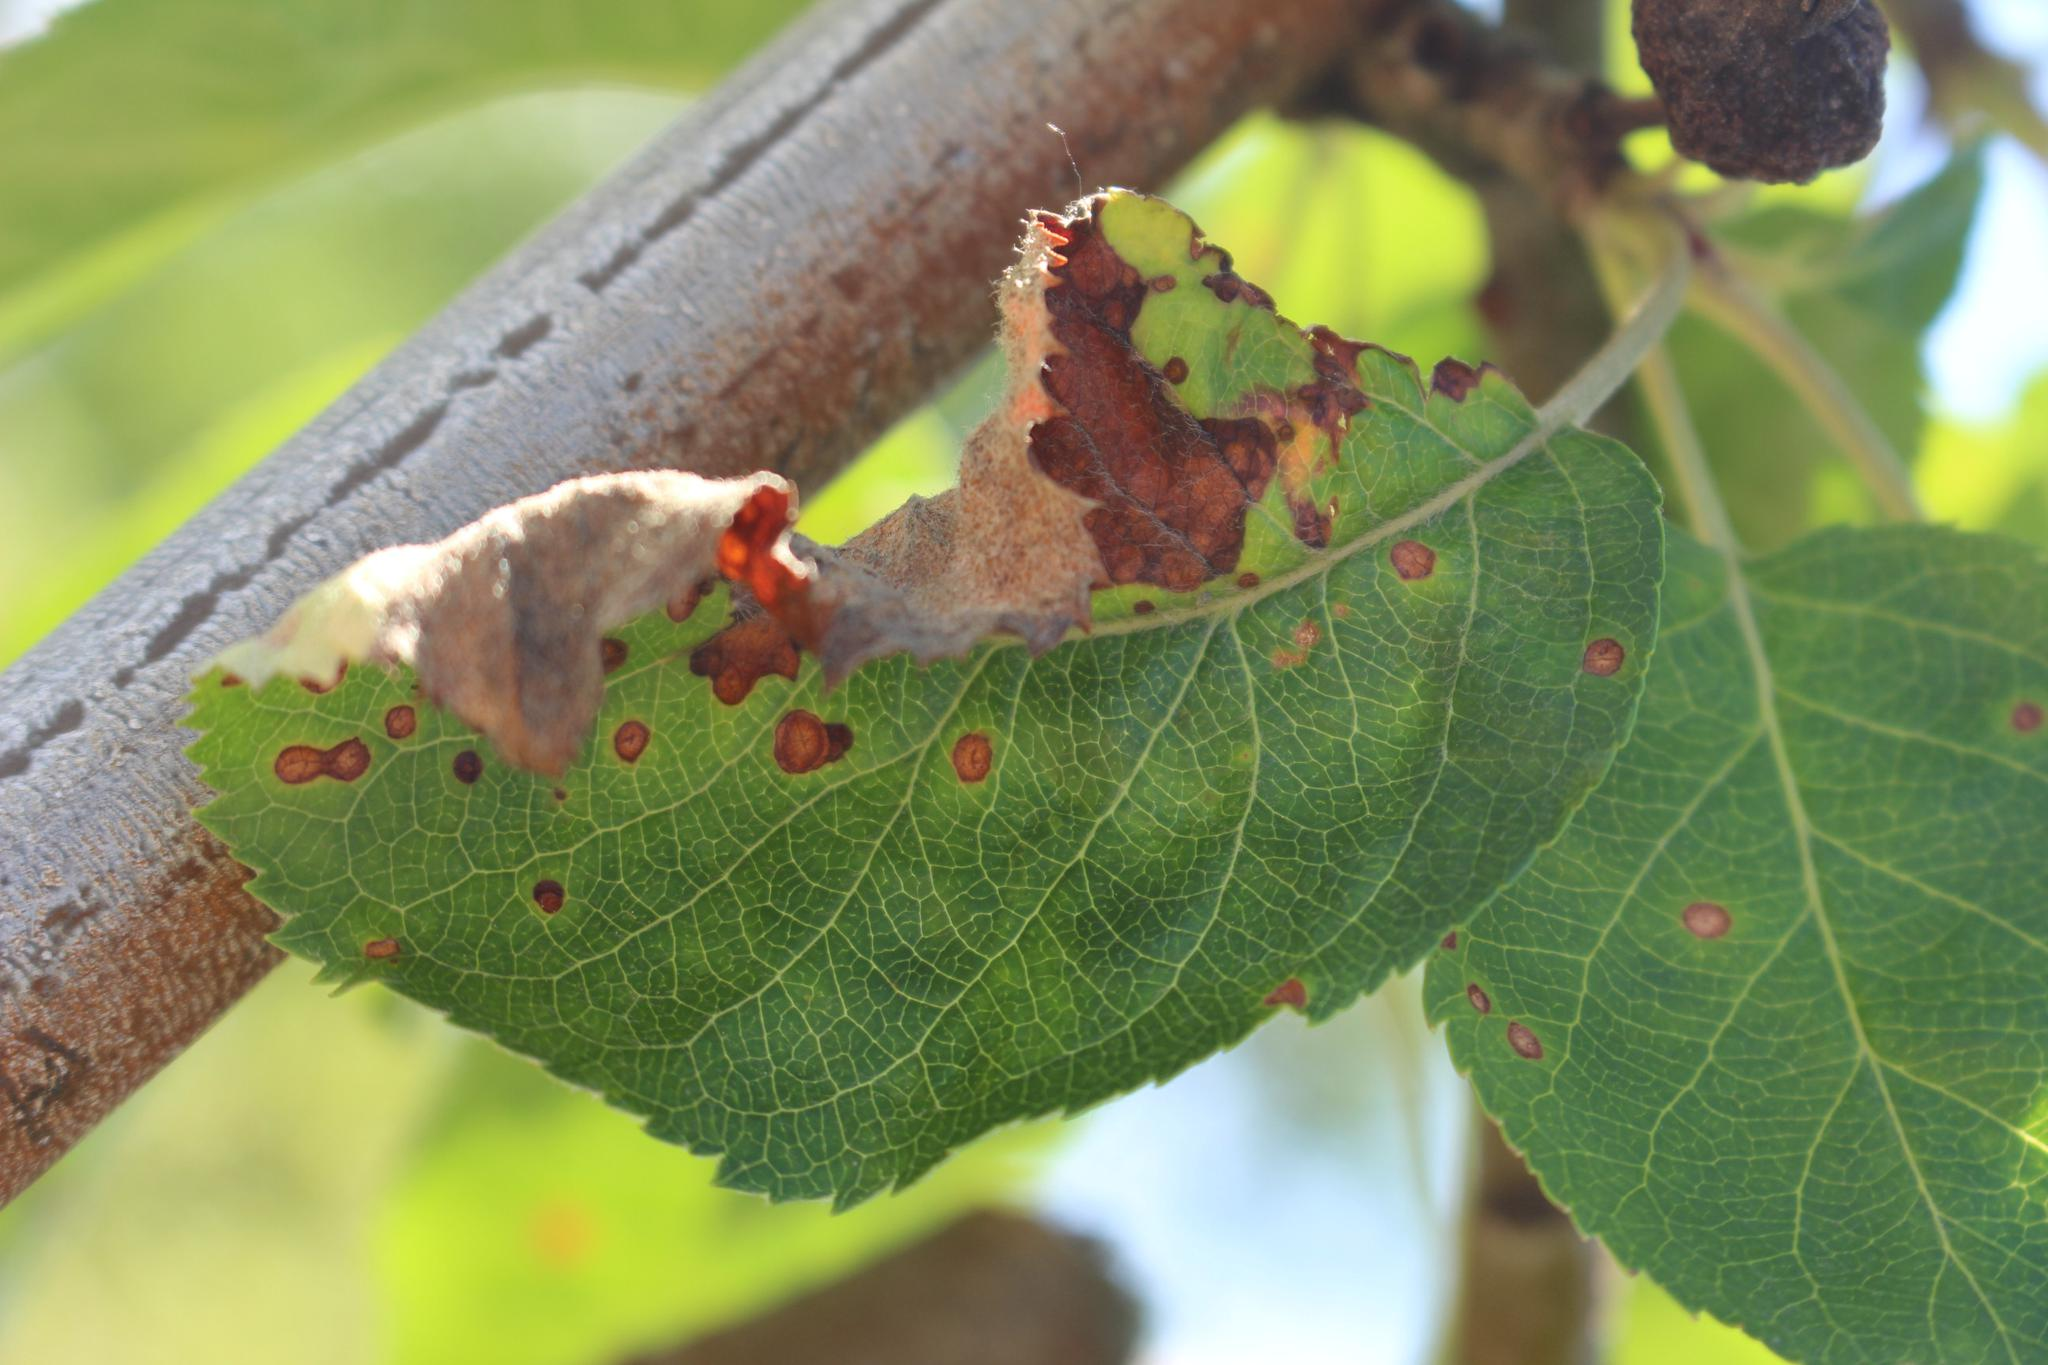
\includegraphics[scale= 0.05]{images/multiple.jpg}  
  \caption{Multiple diseases}
  \label{fig:sub-second}
\end{subfigure}


\begin{subfigure}{.22\textwidth}
  \centering
  % include third image
  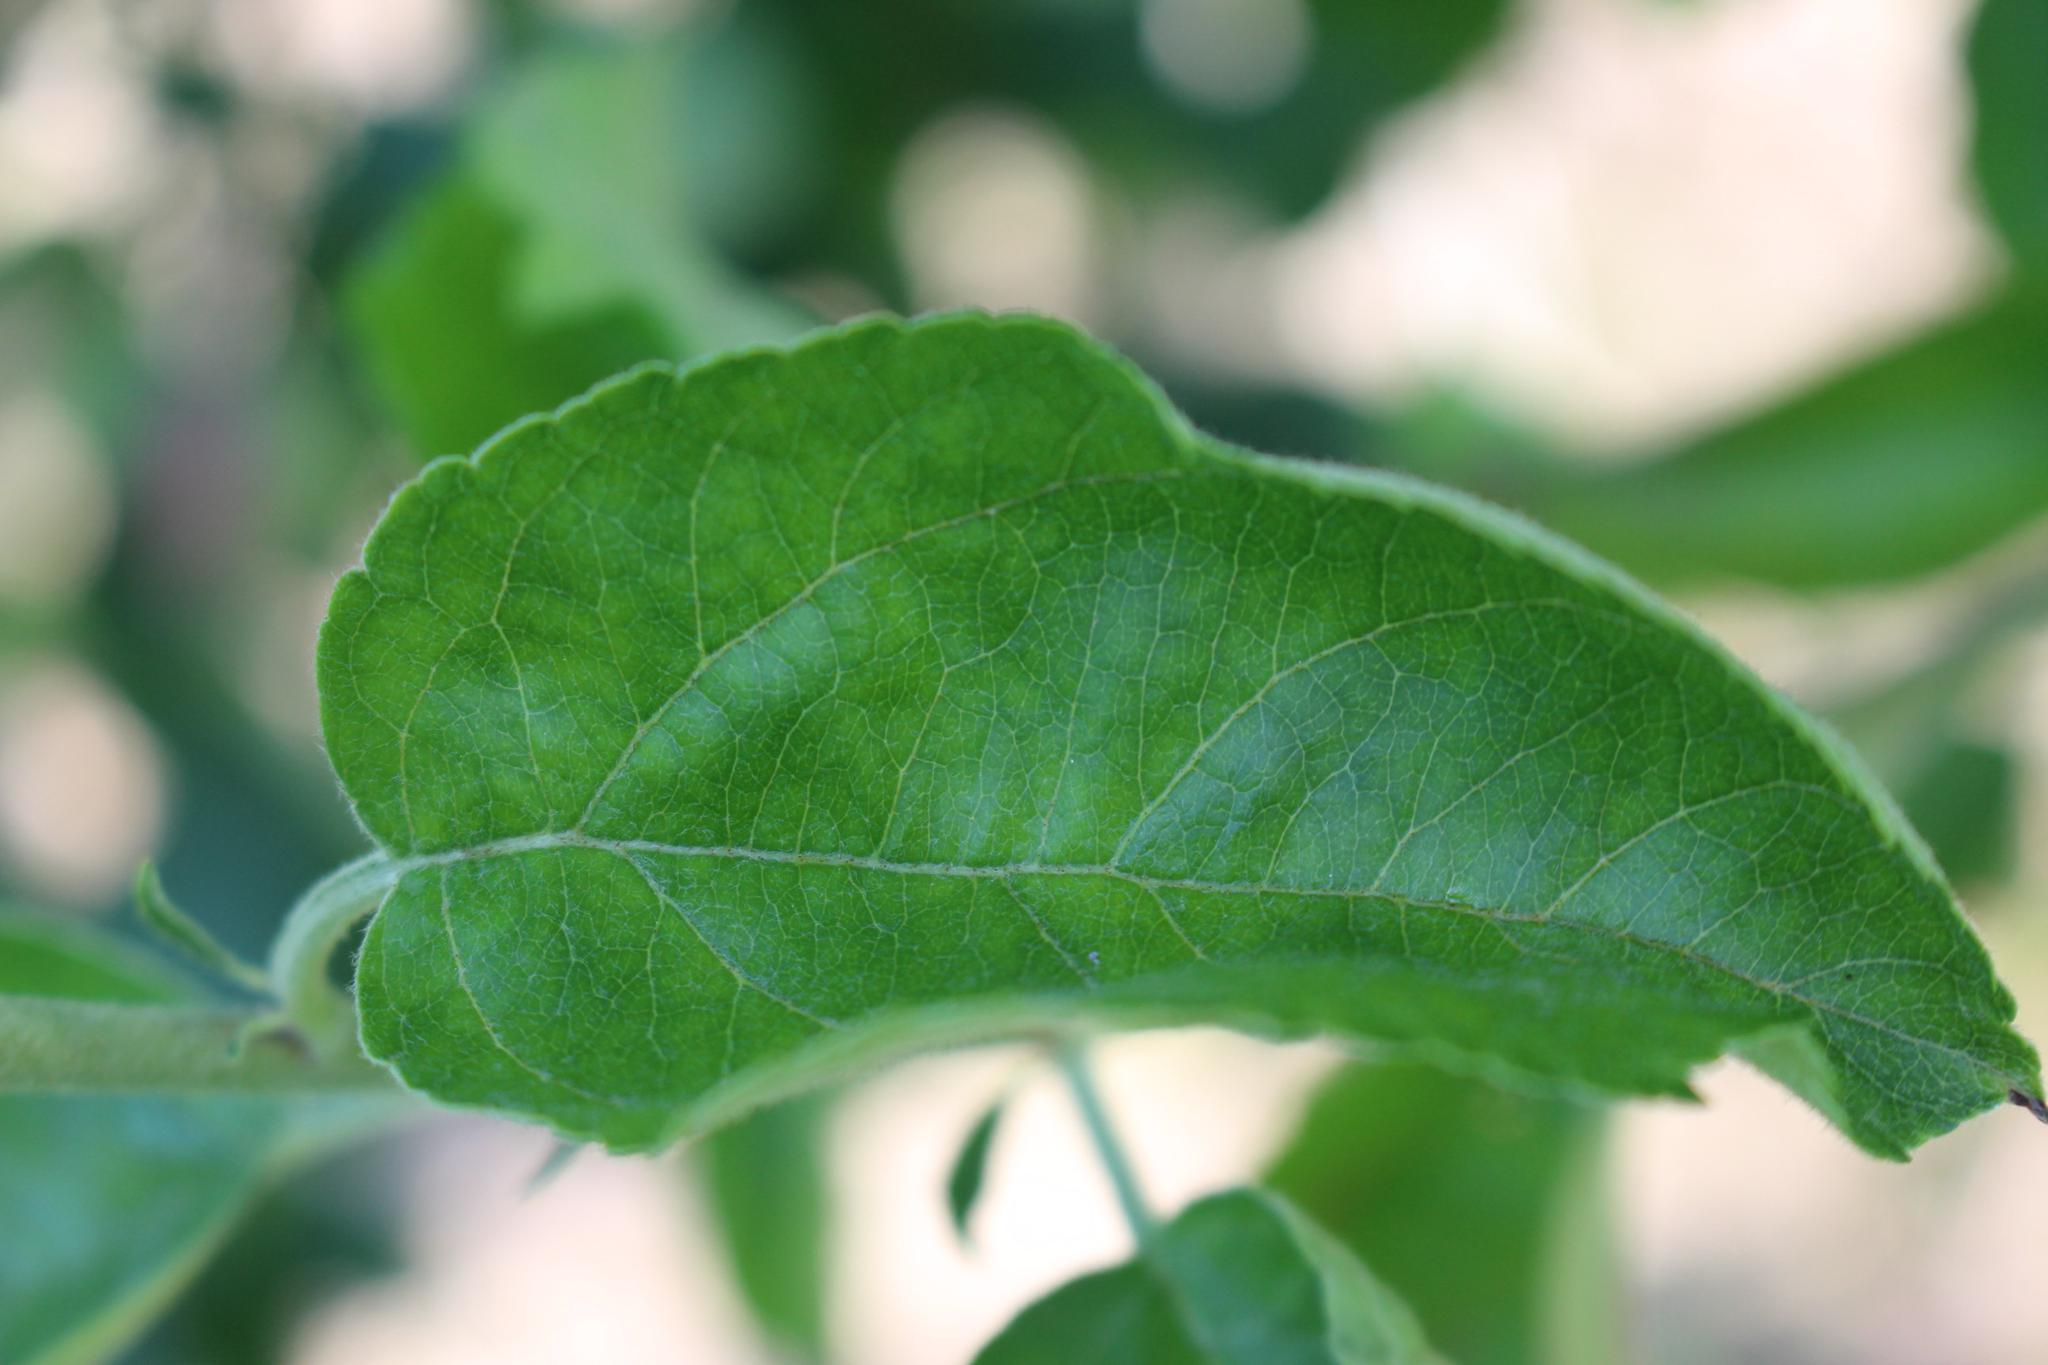
\includegraphics[scale= 0.05]{images/healthy.jpg}  
  \caption{A healthy plant}
  \label{fig:sub-third}
\end{subfigure}
\begin{subfigure}{.22\textwidth}
  \centering
  % include fourth image
  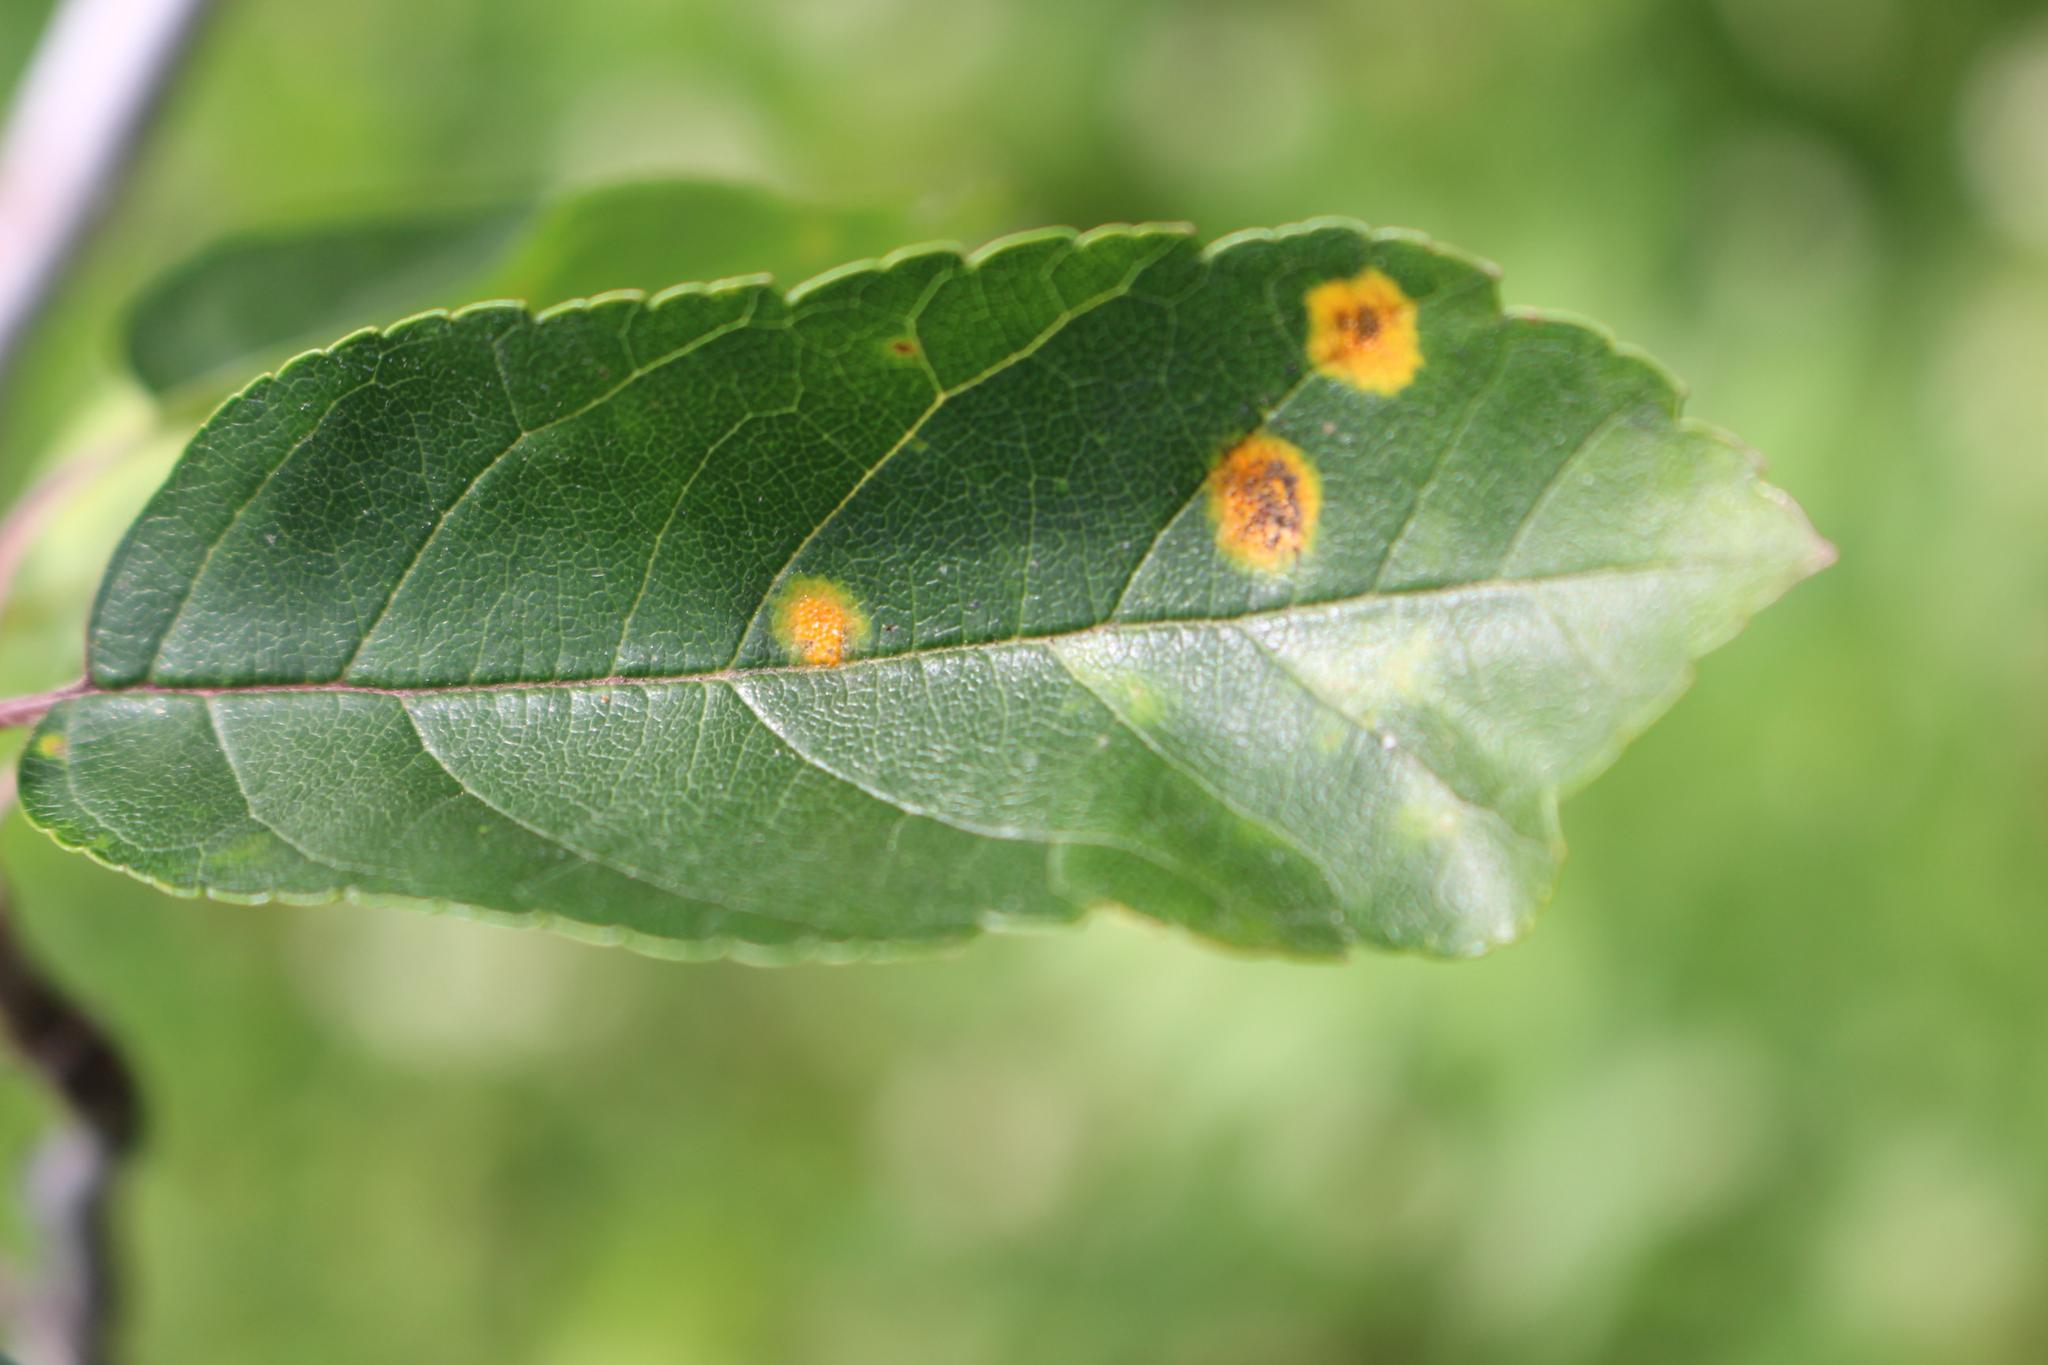
\includegraphics[scale= 0.05]{images/rust.jpg}  
  \caption{Plant with rust}
  \label{fig:sub-fourth}
\end{subfigure}
\caption{Examples of images belonging to each class}
\label{fig:fig}
\end{figure}\\
\\
In the data set a CSV file was available for training. The CSV had the data sorted as one hot encoded labels.
One hot encoding is a group of bits which contains a single '1' bit and all of the rest of the bits are '0'. Each category is converted to a new column and assigned either a '1' or a '0' to define if the image belongs to this category or not.\\
Apart from this a testing CSV file was also available, intended for testing the accuracy of the neural network. After training the neural network was supposed to categorise the images in test data set and one hot encode the results in the CSV file which was then to be uploaded to Kaggle to check the accuracy.    

%-------------------Solution Approach--------------------------------------%
\section{Approach to the solution}
For analyzing visual imagery and classify them convolutional neural networks are widely used. They are ideal for processing 2D images and require very little pre-processing compared to other image classification algorithms which is why for this problem i.e. to classify the images I used a convolutional neural network.

%----------------------CNN-------------------------------------------------%
\subsection{Convolutional Neural Network}
As defined in the famous deep learning book: Convolutional Networks are simply neural networks that use convolution in place of general matrix multiplication in at least one of their layers. \cite{dlbook}\\
Just like a neural network a CNN is made up of an input layer, hidden layers and an output layer. A CNN works by extracting features from the images, which are learned while the network trains. An image is basically a matrix of pixel values. A coloured image is a 3-D Array with a red, green and a blue layer. A CNN consists of Convolutional Layers, ReLU Layers, Pooling Layers and a connected layer. \\
Convolution is used to extract features from the image and is the first step in a CNN. The element which carries out this convolution is called a kernel or a filter. The filter is also selected as a matrix and should have the same depth as the input image. The Kernel or Filter multiplies the values in the filter with the original values in the pixels. These multiplications are then summed up to create a single number. The filter moves across the whole image to carry out this process. The array formed at the end is called a feature map, which is smaller than the original input image.\\
The ReLU layer is the next step to the convolution. In this layer an activation function is applied to set negative values in the feature map to zero. ReLU is chosen as an activation function here because it can train the network faster without causing much changes to the accuracy. \\
Pooling helps with spatial variance i.e. flexibility. We want the network to detect the object no matter where it is located in the picture and pooling helps with it. It also reduces the number of required parameters and the amount of computation. Pooling also helps to control over-fitting. For my network I will be using Max Pooling. Max Pooling grabs the maximum value from each part of the image. This helps to get rid of the information that is not relevant. Even if the image is rotated, the pooled feature will stay the same. This prevents over-fitting. \\
The pooled feature map is then converted to a sequential vector, so the information can be passed on to Artificial Neural Network for further processing. \\
Lastly the Artificial Neural Network combines features into attributes. The error is calculated and back propagated. The weights are adjusted to optimize the performance of the network. \\
After training the network, the fully connected layer uses a classifier in the output layer which usually has softmax as activation function. This uses the features from the previous layer to classify the image. \cite{tds}

%---------------------Solution Implementation------------------------------%
\section{Implementation of the Solution}
\subsection{Pre-processing the data}
To make the data available to the neural network it had to be pre-processed. At first pandas, a library for data manipulation and analysis is used to read the train and testing CSV file.\\
Later Image Data Generator class from Keras library is used which generates batches of tensor image data with real time data augmentation.\\
The method flow from Data Frame in the Image Data Generator class helps to directly pass the previously created Pandas Data Frame which has the mapping between filenames of the images and their labels. At this point the training data is divided into training data and validation data with a ratio of 80:20. 

%---------------------Coding the model-------------------------------------%
\subsection{Coding the Model}
The model consists of stacks of Conv2D and MaxPooling2D Layers. At first the network takes tensors as inputs of shape (ImageSize, ImageSize, 3). The Conv2D Layer creates a Kernel which performs the convolution. The MaxPool2D Layer performs the Max Pooling, where it takes the maximum value over the window defined by pool size. Dropout is then applied to the layers. Dropout is a form of regularization to reduce over fitting. When dropout is applied to the layer, it randomly drops out number of output units from the applied layer during the training process. \\
After 2 of this layers flattening is applied, which flattens the pooled feature map into a sequential vector. \\
To complete the model, the last output tensor from the convolutional base is fed into two Dense layers to perform classification. Dense layers take vectors as input. The first dense layer has ReLU as activation function. As we have 4 output classes, so the final Dense layer has 4 outputs with a softmax activation. \\
The model is then compiled with Adam as optimizer and learning rate of 0.0001. Categorical Cross entropy loss was set as loss function.\\
The model is then trained with 100 Epochs. 


%--------------------Data Augmentation-------------------------------------%
\subsection{Applying Data Augmentation}
As there are small number of training examples available the model did not perform well and achieved an accuracy of 0.729 only. However if data augmentation is applied more training examples can be generated from the existing ones. Random transformations are applied to the existing images. This results in the model not seeing the same image twice during the training process. The model has thus more exposure and can generalise better.\\
The Image Data Generator class can be used to apply augmentation to the images. The images are rotated, resized, flipped and also zoomed to make more training examples from these pre existing images. This resulted in an improvement in the performance and the accuracy came out to be 0.827. 

%----------------------Testing---------------------------------------------%
\subsection{Testing the Model}
The model was tested on the 1821 testing images available in the data set. For this the testing images were passed to the pre-trained model. Which then predicted the class of the images. These predictions were then converted to Boolean data as they had to be one hot encoded. The values were then written to a CSV File using pandas. The file was then uploaded to Kaggle to check the results. 


%----------------------Results---------------------------------------------%
\section{Results}
As explained earlier, the model was at first implemented without data augmentation. This resulted in an accuracy of 0.729. 
\begin{figure}[h]
    \centering
    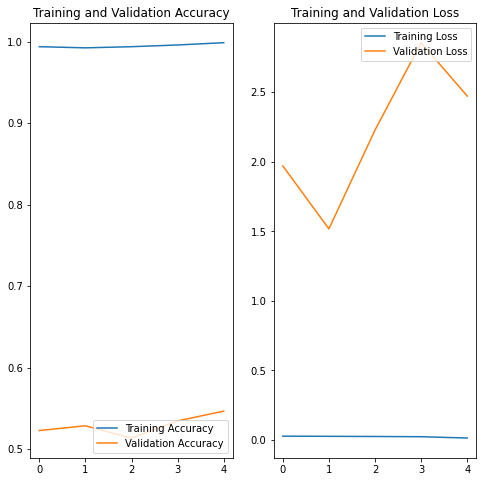
\includegraphics[scale= 0.3]{images/without_augmentation.png}
    \caption{Results without image augmentation}
    \label{fig:without_augmentation}
\end{figure}

After applying image augmentation, the validation accuracy improved and the testing accuracy became 0.829. 
\begin{figure}[h]
    \centering
    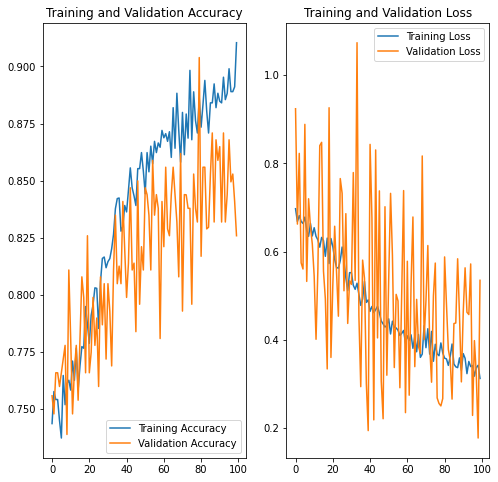
\includegraphics[scale= 0.3]{images/with_augmentation.png}
    \caption{Results with image augmentation}
    \label{fig:with_augmentation}
\end{figure}

%---------------------Improvements----------------------------------------%
\section{Further Improvements}
As seen before the performance of the model is not quite well and can be further improved using the following steps: 
\begin{itemize}
    \item Increasing the number of images in the data set:\\
    Adding more training images for the model to train on can definitely improve the performance and accuracy as the model will have more exposure to different types of data. 
    \item Adding Noise to the network:\\
    Since the data set is quite small, adding noise during training of the neural network can improve the robustness of the model, which helps to reduce over-fitting. \cite{noise}
    \item Using a deeper network topology:\\
    Adding multiple layers to the model can help to learn features at various levels of abstraction. 
\end{itemize}

%----------------------------Ref------------------------------------------%
{\small
\bibliographystyle{ieee}
\bibliography{egbib}
}

\end{document}
